\subsection{Backward Pass}

% \begin{frame}[label=backwardpass_pipeline]{Backward Pass: Pipeline Architecture}
%     \centering
%     \vspace{1.5em}
%     \hspace*{-7.5mm}
%     \resizebox{1.1\linewidth}{!}{%
%     \begin{tikzpicture}[
%         phase/.style={rectangle, draw=blue!80!black, fill=blue!5, thick, rounded corners=4pt, minimum width=2.4cm, minimum height=1.2cm, align=center, font=\scriptsize\bfseries},
%         arrow/.style={-Latex, thick, blue!60!black}
%     ]
%         % --- Phase Nodes (Ordered Left to Right) ---
%         \node[phase] (p1) at (0,0) {Phase 1\\Color Error};
%         \node[phase] (p2) at (3.5,0) {Phase 2\\2D Splat};
%         \node[phase] (p3) at (7.0,0) {Phase 3\\2D Geometry};
%         \node[phase] (p4) at (10.5,0) {Phase 4\\Unprojection};
%         \node[phase] (p5) at (14.0,0) {Phase 5\\Attributes};
        
%         % --- Arrows (Flowing Left to Right) ---
%         \draw[arrow] (p1) -- (p2);
%         \draw[arrow] (p2) -- (p3);
%         \draw[arrow] (p3) -- (p4);
%         \draw[arrow] (p4) -- (p5);
        
%         % --- Top Brackets: Spatial Transformations ---
%         % Phases 1-3: Image Space
%         \draw[gray!80!black, thick] (-1.2, 0.7) -- (-1.2, 0.9) -- (8.2, 0.9) -- (8.2, 0.7);
%         \node[above, font=\small\bfseries] at (3.5, 0.95) {2D Image Space};
        
%         % Phase 4: Image -> View -> World
%         \draw[gray!80!black, thick] (9.3, 0.7) -- (9.3, 0.9) -- (11.7, 0.9) -- (11.7, 0.7);
%         \node[above, font=\small\bfseries] at (10.2, 0.95) {Image $\rightarrow$ View $\rightarrow$ World};
        
%         % Phase 5: World / Latent Space
%         \draw[gray!80!black, thick] (12.8, 0.7) -- (12.8, 0.9) -- (15.2, 0.9) -- (15.2, 0.7);
%         \node[above, font=\small\bfseries] at (14.0, 0.95) {3D World Space};
        
%         % --- Bottom Brackets: GPU Architecture Modes ---
%         % Phases 1-3: Pixel-based
%         \draw[gray!80!black, thick] (-1.2, -0.7) -- (-1.2, -0.9) -- (8.2, -0.9) -- (8.2, -0.7);
%         \node[below, font=\small\bfseries] at (3.5, -0.95) {One GPU Thread per Pixel};
        
%         % Phases 4-5: Per-Gaussian
%         \draw[gray!80!black, thick] (9.3, -0.7) -- (9.3, -0.9) -- (15.2, -0.9) -- (15.2, -0.7);
%         \node[below, font=\small\bfseries] at (12.25, -0.95) {One GPU Thread per 2D/3D Gaussian};
        
%     \end{tikzpicture}%
%     }
    
% \end{frame}

\begin{frame}{Backward Pass: Architecture \& Gradient Flow}
    \centering
    \resizebox{\linewidth}{!}{%
        \begin{tikzpicture}[
            % Styles for variables and arrows
            var/.style={circle, draw=blue!60!black, fill=blue!10, thick, minimum size=1.1cm, inner sep=0pt, font=\small\bfseries},
            varfirst/.style={circle, draw=blue!60!black, thick, minimum size=1.1cm, inner sep=0pt, font=\small\bfseries},
            endvar/.style={circle, draw=green!60!black, fill=green!10, thick, minimum size=1.1cm, inner sep=0pt, font=\small\bfseries},
            arrow/.style={-Latex, thick, blue!70!black},
            header/.style={font=\footnotesize\bfseries, text=gray, align=center}
        ]
            % --- Top Brackets: Spatial Transformations ---
            % Phases 1-3: Image Space
            \draw[gray!80!black, thick] (-1.5, 4.0) -- (-1.5, 4.2) -- (11.1, 4.2) -- (11.1, 4.0);
            \node[above, font=\small\bfseries] at (5, 4.25) {2D Image Space};
            
            % Phase 4: Image -> View -> World
            \draw[gray!80!black, thick] (11.3, 4.0) -- (11.3, 4.2) -- (14.3, 4.2) -- (14.3, 4.0);
            \node[above, font=\scriptsize\bfseries] at (12.8, 4.25) {Image $\rightarrow$ View $\rightarrow$ World};
            
            % Phase 5: World Space
            \draw[gray!80!black, thick] (14.5, 4.0) -- (14.5, 4.2) -- (17.5, 4.2) -- (17.5, 4.0);
            \node[above, font=\small\bfseries] at (16.0, 4.25) {3D World Space};

            % --- Column Headers ---
            \node[header] at (0, 3.2) {Loss};
            \node[header] at (3.2, 3.2) {Phase 1\\Loss to Pixel\\ Color Corr.};
            \node[header] at (6.4, 3.2) {Phase 2\\Pixel Color Corr.\\ to 2D Splat};
            \node[header] at (9.6, 3.2) {Phase 3\\2D Splat to\\ 2D Geometry};
            \node[header] at (12.8, 3.2) {Phase 4\\2D Geometry to\\ 3D Geometry};
            \node[header] at (16.0, 3.2) {Phase 5\\3D Geometry to\\ 3D Gaussian Attributes};
            
            % --- Vertical Separators ---
            \foreach \x in {1.6, 4.8, 8.0, 11.2, 14.4} {
                \draw[dashed, gray!30] (\x, 3.8) -- (\x, -3.8);
            }

            % --- Nodes ---
            \node[varfirst] (L) at (0, 0.3) {$L$};
            \node[var] (Cp) at (3.2, 0.3) {$C_p$};
            
            \node[endvar] (ci) at (6.4, 1.8) {$c_i$};
            \node[var] (alpha) at (6.4, -0.7) {$\alpha_i$};
            
            \node[var] (mu2D) at (9.6, 0.8) {$\mu_{2D}$};
            \node[var] (Sigma2D) at (9.6, -0.7) {$\Sigma_{2D}$};
            \node[var] (o) at (9.6, -2.2) {$o$};
            
            \node[endvar] (mu3D) at (12.8, 0.8) {$\mu_{3D}$};
            \node[var] (Sigma3D) at (12.8, -0.7) {$\Sigma_{3D}$};
            
            \node[endvar] (sraw) at (16.0, 0.1) {$s_{raw}$};
            \node[endvar] (qraw) at (16.0, -1.5) {$q_{raw}$};
            \node[endvar] (oraw) at (16.0, -2.9) {$o_{raw}$};
            
            % --- Edges (Gradient Flow) ---
            \draw[arrow] (L) -- (Cp);
            \draw[arrow] (Cp) -- (ci);
            \draw[arrow] (Cp) -- (alpha);
            \draw[arrow] (alpha) -- (mu2D);
            \draw[arrow] (alpha) -- (Sigma2D);
            \draw[arrow] (alpha) -- (o);
            \draw[arrow] (mu2D) -- (mu3D);
            \draw[arrow] (Sigma2D) -- (Sigma3D);
            \draw[arrow] (Sigma3D) -- (sraw);
            \draw[arrow] (Sigma3D) -- (qraw);
            \draw[arrow] (o) -- (oraw);
            
            % --- Legend ---
            \node[var, minimum size=0.5cm] at (4.0, -4.0) {};
            \node[right, font=\scriptsize] at (4.3, -4.0) {Intermediate Gradient};
            
            \node[endvar, minimum size=0.5cm] at (9.5, -4.0) {};
            \node[right, font=\scriptsize] at (9.8, -4.0) {Final Attribute Gradient};

            % --- Bottom Brackets: GPU Architecture Modes ---
            % Phases 1-3: Pixel-based
            \draw[gray!80!black, thick] (-1.5, -4.5) -- (-1.5, -4.7) -- (11.1, -4.7) -- (11.1, -4.5);
            \node[below, font=\small\bfseries] at (5, -4.75) {One GPU Thread per Pixel};
            
            % Phases 4-5: Per-Gaussian
            \draw[gray!80!black, thick] (11.3, -4.5) -- (11.3, -4.7) -- (17.5, -4.7) -- (17.5, -4.5);
            \node[below, font=\small\bfseries] at (14.4, -4.75) {One GPU Thread per 2D/3D Gaussian};
            
            % --- Slide 2 Overlay: Loss Formula ---
            \node<2->[
                align=center, 
                anchor=north west,
                text width=4.7cm
            ] at (-1.5, 3) {
                $$\darkmathhighlight{ L = (1-\lambda)\cdot\mathcal{L}_1 + \lambda\cdot\mathcal{L}_{D-SSIM}}$$
            };

            \node<2->[
                align=center, 
                anchor=north west,
                text width=4.7cm % Required when using display math inside a TikZ node
            ] at (-0.85, 2.1) {
                $$\darkmathhighlight{\frac{\partial L}{\partial C_p}}$$
            };

            \node<3->[
                align=center, 
                anchor=north west,
                text width=4.7cm % Required when using display math inside a TikZ node
            ] at (01.2, 0) {
                $$\darkmathhighlight{
             \frac{\partial L}{\partial \alpha_i} = 
             \frac{\partial L}{\partial C_p} \cdot \frac{\partial C_p}{\partial \alpha_i}}$$
            };

        \end{tikzpicture}%
    }

    \pdfcomment[opacity=0]{
        - as with the forward pass, we subdivide the backward pass as well, this time into five phases. \textCR
        - In principle we are moving backwards through the calculations made in the forward pass, starting with the color error \textCR
        - This then propagates through 2D Gaussian splats and geometry, is being unproject into 3D space and finally we are adjusting the 3D Gaussian's attributes
    }
    \pdfcomment[opacity=0]{
        - Training compares the rendered image with the original input image using a weighted combination \textCR
        - L1 calculates the absolute pixel-wise error, while D-SSIM acts as a structural regularizer \textCR
        - what is D-SSIM (a structual similarity index)\textCR
        - explain resulting gradient for phase 1
    }
    \pdfcomment[opacity=0]{
        - In phase 2 we can see that we can use the color error gradients to calculate the color and opacity gradients using the chain rule (mark elements) \textCR
        - This means the gradients adjust the color based on its contribution or the opacity if the pixel error is reduced more effectively by the Gaussians color than the accumulated background color behind it. \textCR
        - (transition to pipeline)
    }
    \pdfcomment[opacity=0]{
        - Phase 3: The opacity gradients are used to adjust the physical properties of the 2D Gaussians \textCR
        - Phase 4: Unprojection: The 2D gradients are unprojected back into 3D space, translating the 2D adjustments into 3D center movements and 3D volume changes. \textCR
        - Phase 5: The gradients flow backward through the 3D covariance matrix assembly.\textCR
    }
\end{frame}

\begin{frame}{Adaptive Density Control}
    \begin{itemize}
        \justifying
        \item Steps in every 100 iterations to counter over-reconstruction (covering too much geometry) and under-reconstruction (too few Gaussians).
        %\item \textbf{Splitting:} Over-reconstructing Gaussians are split into two smaller ones.
        %\item \textbf{Cloning:} Under-reconstructing Gaussians are cloned.
        %\item \textbf{Pruning \& Opacity Reset:} 3D Gaussians with extremely low opacity or unbound scale are routinely deleted.
    \end{itemize}

    \vspace{2mm}
    {
        \centering
        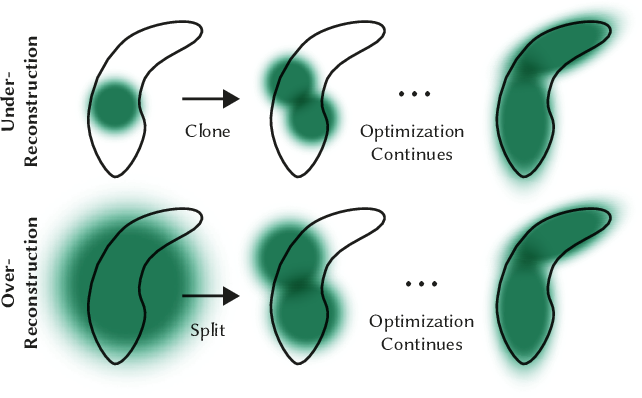
\includegraphics[width=0.65\linewidth]{../figures/6-Figure4-1.png}\\
        \centering \tiny Graphic extracted from Kerbl et al. \cite{kerbl3DGaussianSplatting2023}
    }

    \pdfcomment[opacity=0]{
        - housekeeping \textCR
        (jump to training cycle directly) \textCR
        - mention novel view synthesis
    }
\end{frame}

\begingroup
    \addtocounter{framenumber}{-1}
    \againframe{training_cycle}
\endgroup

